\documentclass{article}
\usepackage{graphicx}
\usepackage{subfig}
\usepackage{amsmath}
\begin{document}
\section{Related Work}
\subsection{Basic concepts}
\subsubsection{Message Authentication}
The message authentication system aims to provide protection on the integrity of messages. Assume the sender A sends message M to receiver B,the message authentication system be eligible to examine the modification on M. The concept of message authentication system is expressed in Figure 1. The sender uses the message as input to the tag generation system(TG$_K$(M)) to generate a short information block called tag. The message is concatenated with tag and transmitted to the receiver. Before the receiver accept the message M, M and its tag T are sent to the verification system(VF$_K$(M,T)). If the output of verification system is 1, that means the M and T are not matched, otherwise the message M is accepted by the receiver. 
\begin{figure}[htbp]
\centering
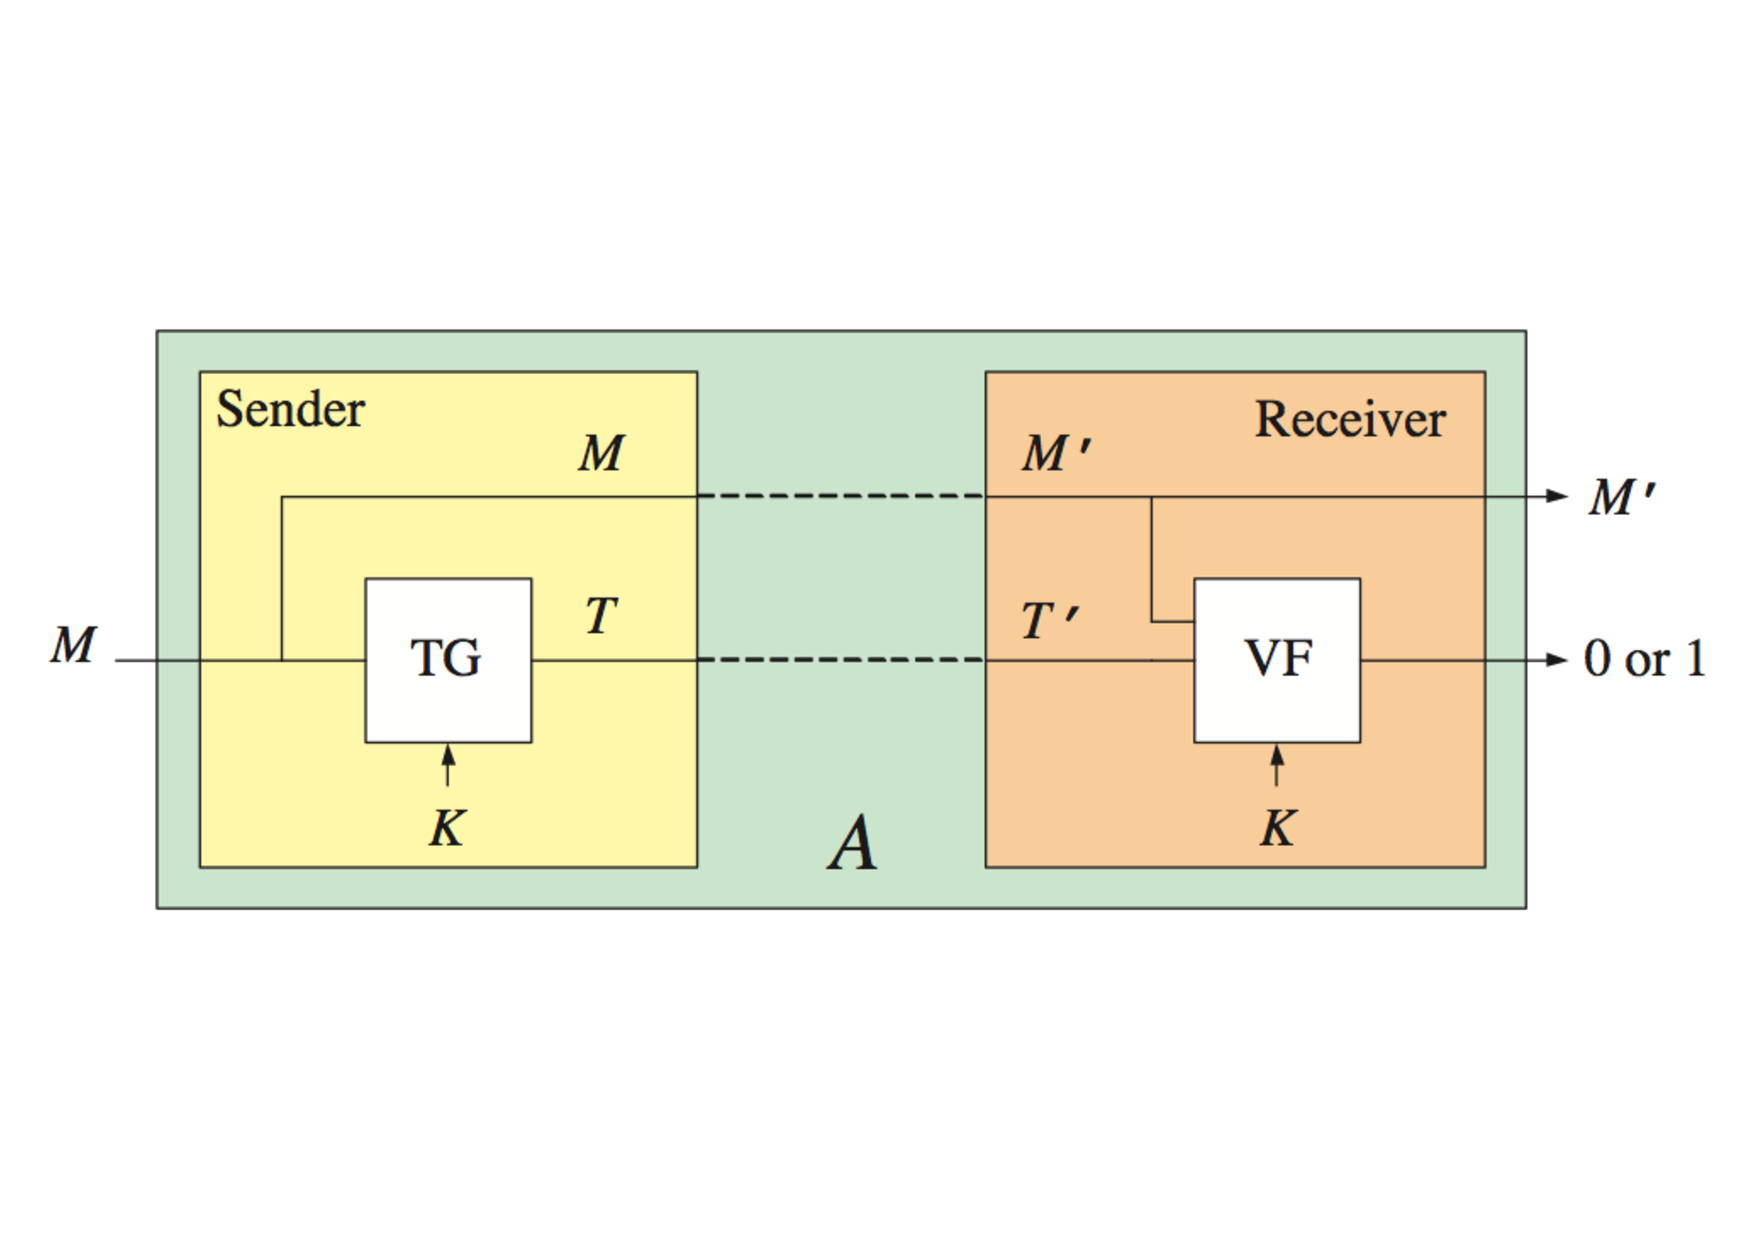
\includegraphics[scale=0.4]{./diagram/ma.pdf}
\caption{The Concept of Message Authentication System}
\label{fig:1 }
\end{figure}
\paragraph{Common Message Authentication Systems}
The Message Authentication Code(MAC) is a common message authentication system. The concept of MAC scheme can be seen in Figure 2. In a deterministic MAC scheme, the verification system adopts the same key used in tag generation system. In the verification part of a MAC scheme, the tag T1 of message M is computed and compared with the tag T concatenated with the M. If T1=T then the verification system output 1 and the receiver accepts M, otherwise the verification system output 0. 
The early designed MAC schemes are deterministic, which means neither the sender nor the receiver needs to maintain a state used in tag generation. Latter some MAC designs adopt a state maintained by the user in the tag generation, such as the GMAC \cite{gcm} and Cost-Effective Tag Design \cite{cetd}.  

Digital signature is another kind of message authentication system. The signature generation uses a private key while the message verification stage uses public key. The digital signature system can assure non-repudiation of the message protected while MAC schemes can not.
\begin{figure}[htbp]
\centering
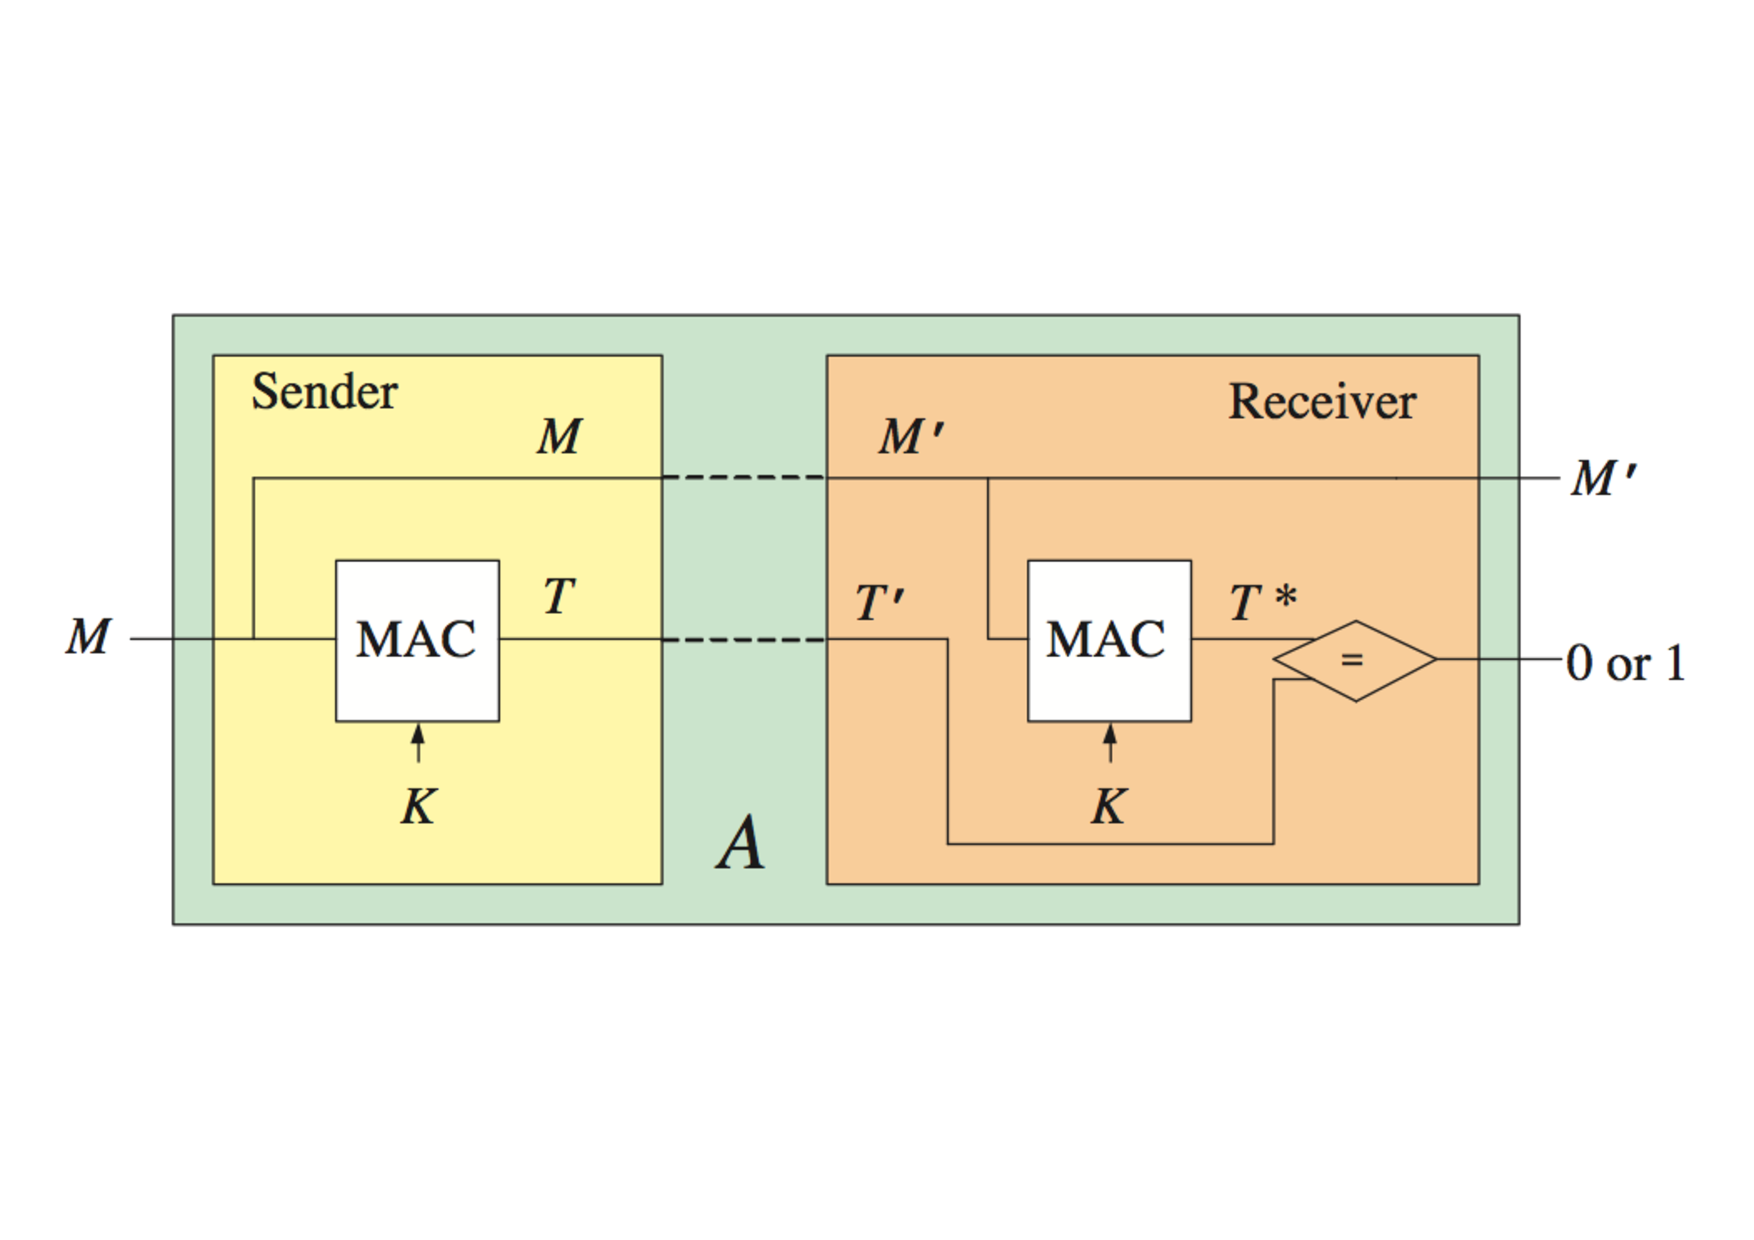
\includegraphics[scale=0.4]{./diagram/MAC.pdf}
\caption{Message Authentication Code(MAC)}
\label{fig:2 }
\end{figure}
\subsubsection{The Security of MAC schemes}
\paragraph{The forgery attacks}
When attacking a message authentication system, the adversary try to send a pair(M,T) to the receiver to make VF$_k$(M,T)=1 while M did not originate with the legal sender. The fake pair(M$_f$,T$_f$) that makes VF$_k$(M$_f$,T$_f$)=1 is called a forgery from the adversary. A successful forgery attack indicates that the adversary has made a forgery. 
The purpose of a message authentication system is preventing the receiver to accept the message from unauthorized senders, such as an adversary. The quantitative property of a secure message authentication system is the low probability for an adversary to make a successful forgery attack with the limited resource.
\paragraph{Chosen-message attacks}
A strong type of attack that an adversary can conduct on the message authentication system is the adaptive chosen-message attack, marked as uf-cma. When doing uf-cma, the adversary chooses its own input message M and acquires the relative tag T. The adversary try to find the weakness in the design of message authentication system by analyzing the pairs(M,T) of his choice. The uf-cma provides the adversary with the most capability to succeed in the forgery attack. The probability that an adversary conducts a successful forgery attack after limited times of uf-cma is adopted as the basic quantitative security property of a message authentication in cryptography. This fact was also mentioned in \cite{Rogaway2011}.
\paragraph{The Security Notions of MAC schemes}
The formalised quantitative notion of the security of a MAC scheme was introduced by Bellare et al. in \cite{cbc1994}. This notion follows the security notion of digital signature introduced in \cite{signature}. The successful forgery on a MAC scheme from an adversary A is measured by a experiment called Forgery(MAC,A). In Forgery(MAC,A),  
the adversary A is provided a black-box access to the tag generation system TG$_K$(). When TG$_K$() takes an input message M$_i$, it returns tag T$_i$ to A. A conducts uf-cma by keep sending the message queries M$_i$ and observes the relative tag T$_i$ for limited times. On the other hand, A is provided a black-box access to the verification system VF$_K$(). When A sends a pair(M$_j$,T$_j$) to VF$_K$(), the VF$_K$() computes the tag T of M$_j$ and compares T with T$_j$. If T=T$_j$ then VF$_K$()=1 otherwise 0. If A sends a pair(M,T) that makes VF$_K$() outputs 1 while M has not appeared in the previous queries of uf-cma, then A succeeds a forgery attack and Forgery(MAC,A)=1.

The quantitative security notion of a MAC scheme is forgery probability, expressed as Forgery$_MAC$=Pr[Forgery(MAC,A)=1].
\paragraph{The Correlation between Security and Randomness}
Goldreich, Goldwasser, and Micali asserted in \cite{prf} that any good pseudorandom function(PRF) is a secure MAC scheme under the quantitative security notion. Bellare, Kilian and Rogaway proved this assertion in \cite{cbc1994} saying that if a system behave like a pseudoranom function, this system is a secure MAC scheme if meeting the requirements on domain and range of MAC schemes. Based on these two reduction of security notion, latter researches on security evaluation of MAC schemes posted their focuses on analyzing whether the MAC scheme evaluated behaves like a PRF.
\paragraph{The Randomness of a MAC scheme}
The definition of PRF was introduced in \cite{prf} indicating that PRF could not be distinguished from a ideal random function each bit of whose output was a coin flip. To define how closely a MAC scheme behaves like a PRF, Bellare et al. provided a quantitative notion in \cite{cbc1994} named Adv$^{PRF}_{MAC}$(), which was based on the concept of distinguisher introduced in\cite{prf}. 

Let F$_0$ and F$_1$ be two function with a common domain D and a common range R. A distinguisher A for F$_0$ versus F$_1$ is an adverary A that has access to a black box named oracle f:D->R. After accessing the oracle f, A computes a bit. Assume the function stored in the oracle f is X and A guesses that X is in the oracle, then A computes 1 otherwise 0. The the advantage of A in distinguishing F$_0$ from F$_1$ is expressed as Adv$^{F0}_{F1}$=Pr[f$\stackrel{R}{\longleftarrow}$F0:A$^{F0}$=1]-Pr[f$\stackrel{R}{\longleftarrow}$F1:A$^{F1}$=1]. Pr[f$\stackrel{R}{\longleftarrow}$F0:A$^{F0}$=1] means when the content of oracle f is F0, A guesses that F0 is in oracle then output 1.

We can see that if F0 behaves much like F1, it is hard for A to distinguish between F0 and F1 then Adv$^{F0}_{F1}$ is very small. This case is adopted by Bellare et al. in the quantitative notion of randomness of a MAC scheme. If the randomness of a MAC scheme is good, then the MAC scheme behaves like a PRF and Adv$^{[PRF]}_{MAC}$ is small. 



\subsection{The deterministic MAC schemes}
\paragraph{Properties of the Deterministic MAC Schemes}
The early MAC schemes are deterministic systems, which means the sender and receiver do not need to maintain a state for tag generation. The deterministic MAC schemes are symmetric system as the key used by the TG and VF is the same one. Some of the deterministic MAC schemes are designed based on block cipher, keyed cryptographic hash functions or other cryptographic primitives.
\subsubsection{Security Evaluation of the Deterministic MAC schemes}
\paragraph{The Computational approach of Security evaluation for MAC schemes}
The approach adopted by researchers in analyzing the security of deterministic MAC schemes can be described as the following procedure: expressed Adv$^{PRF}_{MAC}$ with a equation consist of Adv$^{PRP}_{E(K)}$, where E(k) represents the block cipher with key k used in the MAC scheme. Hence the quantitative security result Adv$^{PRF}_{MAC}$ is based on the result Adv$^{PRP}_{E(K)}$, and Adv$^{PRP}_{E(K)}$ is defined by the computational assumption in cryptography, this approach in computing the quantitative security result is called computational approach by some researchers.

PRP represent pseudorandom permutation, which is introduced by Luby and Rackoff`in \cite{PRP} claiming that a good block cipher should
behave like a pseudorandom permutation(PRP) whose output should be uniformly and randomly generated and their values
should be distinct if the inputs are distinct.
According to the assumption in cryptography, the ideal block cipher behaves exactly as pseudorandom permutation. The quantitative security analysis of deterministic MAC schemes are based on this assumption in the calculation of Adv$^{PRF}_{MAC}$.
\paragraph{The Experiment based Randomness Evaluation}
According to the computational approach of security analysis on deterministic MAC schemes, the security of a MAC scheme is based the assumption that the block cipher or other cryptographic primitives(such as cryptographic hash function in HMAC) show high level randomness. 

There have been researches on designing tools for randomness evaluation to provide empirical evidence of randomness assumption in security analysis.
Early works included DIEHARD suite, Crypt-XS, The NIST
Statistic Test Suite(short for the NIST suite) and so on. Soto introduced a randomness testing suite designed by the National Institure of Standard Technology in \cite{Soto1999}. The properties of the NIST suite is analyzed in detailed in \cite{NIST_suite} together with the instruction on using the NIST suite for randomness testing.
The majority advantages of NIST suite are:
\begin{itemize}
	\item The NIST suite covers most hard-to-pass tests for binary sequences
	mentioned in previous suites(such as DIEHARD or Crypt-XS)
	\item The purpose of each statistic tests is explained in detail to show
	what kind of defect of the input is examined.
	\item NIST suite has been used in candidate selection of Advanced Encryption
	Standard(AES). The results acquired under the result collection and analysis instruction of NIST suite is
	convincing.
\end{itemize}
The NIST suite has be adopted in the candidate selection of Advanced Encryption Standard(AES). The detailed information about selection is discussed in \cite{candidate_test,final_test}. 
\subsubsection{Iterated MAC schemes}
\begin{figure}[htbp]
\centering
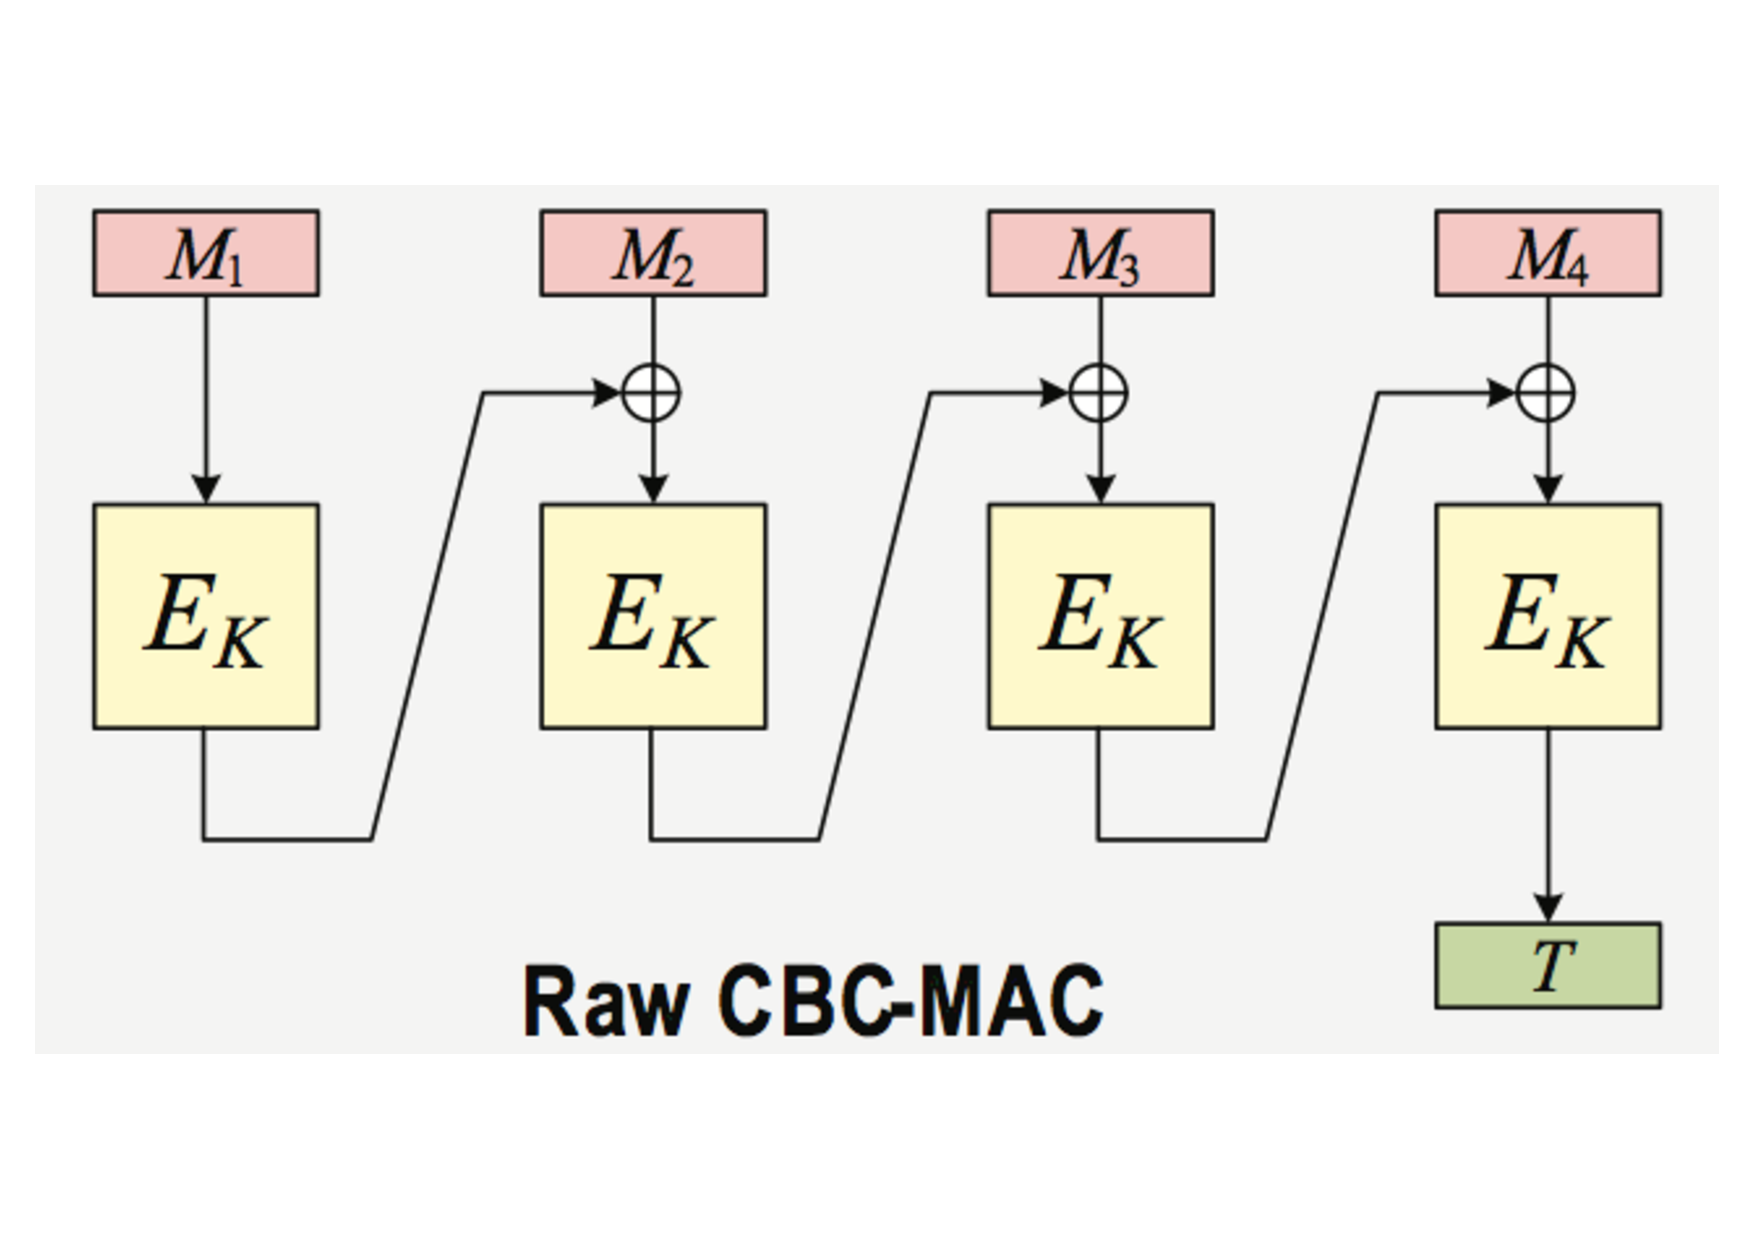
\includegraphics[scale=0.3]{./diagram/cbc-mac.pdf}
\caption{The Raw CBC-MAC}
\label{fig:3 }
\end{figure}
The research on iterated MAC schemes started from the raw CBC-MAC expressed in Figure 3.
\paragraph{Raw CBC-MAC}
The cryptographic primitive used in the raw CBC-MAC scheme is block cipher.  
The raw CBC-MAC is a secure MAC for only fixed length inputs. Assume the tag T of message M from CBC-MAC can be expressed as T = CBC-MAC$_k$(M), for another input M$\|$(M$\oplus$T), the tag T1=CBC-MAC(M$\|$(M$\oplus$T))=T. This attack indicates that the raw CBC-MAC is vulnerable if the input length is not fixed.
Besides the vulnerability when the input length is not fixed, the raw CBC-MAC scheme suffers birthday attack, means the adversary needs only 2$n/2$ input queries to succeed a forgery. 

Bellare et al. provided the original security evaluation on raw CBC-MAC\cite{cbc1994}. The conclusion is that if the adversary A is allowed to conduct arbitrary fixed length queries for q time, the probability that A succeeds in a forgery after the queries can be expressed with the queries times q and the computational assumption of block cipher used. Their quantitative conclusion showed that the forgery probability is very small.

\paragraph{EMAC}
The motivation of EMAC design is the problem that the raw CBC-MAC is secure only for fixed length inputs. 
EMAC is a optimized version of raw CBC-MAC providing security for arbitrary length inputs. The in the EMAC scheme, the final message block in the input is processed by a padding function to ensure that all the input blocks have the same length. Then raw CBC-MAC is applied applies and the result is encrypted by a the same block cipher in raw CBC-MAC with a different key. 

Petrank and Rackof provided the original security evaluation of EMAC in \cite{emac}. The EMAC is secure for arbitrary length inputs under the security notion if the block cipher meets the related computational assumptions. However, the EMAC still suffers the birthday attack.
\subsubsection{CMAC: Optimized CBC-MAC}
\begin{figure}[htbp]
\centering
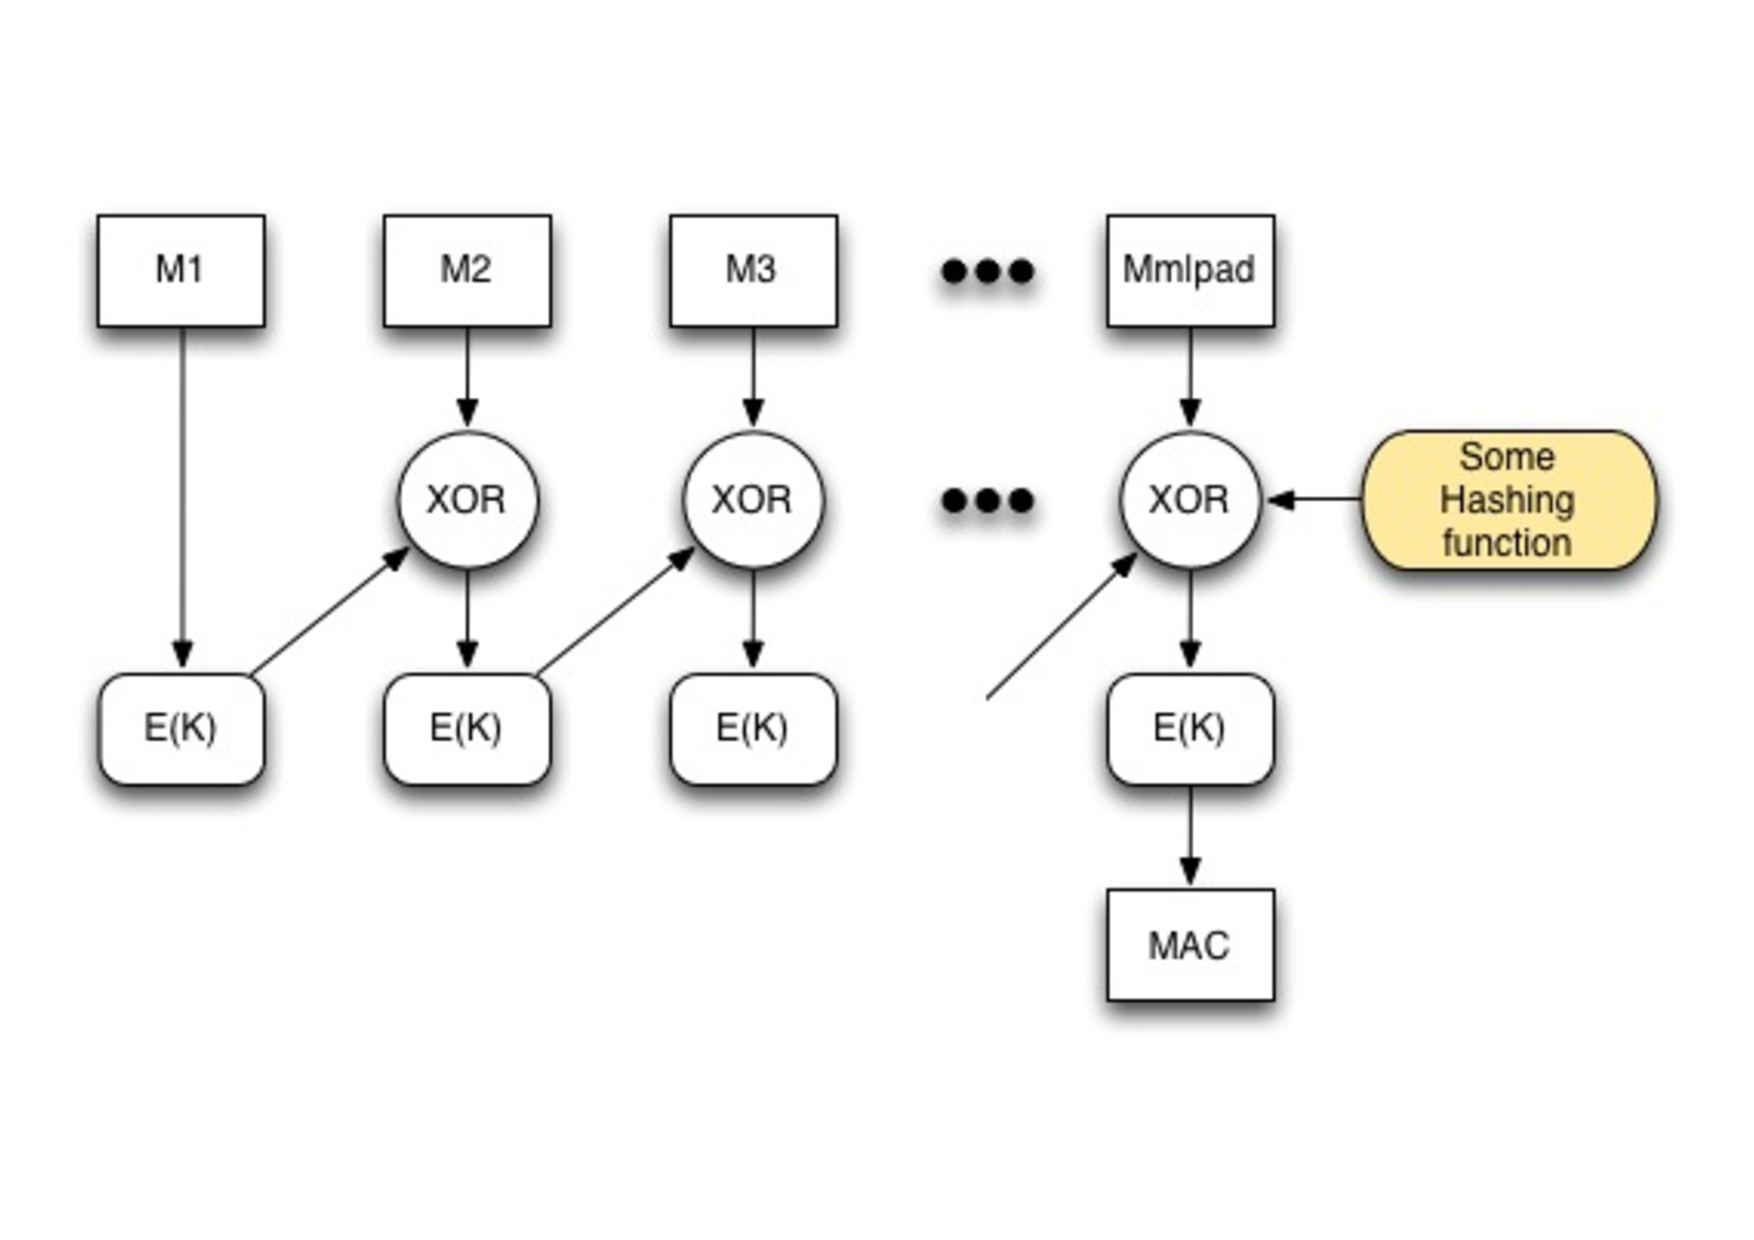
\includegraphics[scale=0.3]{./diagram/cmac.pdf}
\caption{The class of CMAC}
\label{fig:4 }
\end{figure}
Hence the raw CBC-MAC is vulnerable if the input length is not fixed, a class of MAC schemes named CMAC are developed to provide security for arbitrary length of inputs. The structure of the  variants of CMAC is modeled in Figure 4.
\paragraph{XCBC: three key version of CMAC }
Black and Rogaway introduced a optimized version of EMAC called XCBC in \cite{xcbc}.
There are two motivations of XCBC scheme: providing security for arbitrary length input; eliminate unnecessary padding operation on the input blocks in EMAC.

The XCBC scheme is a refined version of original EMAC. The contributions of XCBC scheme compared with the EMAC are: extending the domain to full domain; the block ciphers used in processing m input blocks is m other than m+1 in EMAC; all the block cipher in XCBC share a same key, the additional two keys are used to do exclusively or operation with the final input block,this design has faster processing speed.   

Black and Rogaway provided a original security analysis based on computational approach of XCBC scheme in \cite{xcbc}. Their quantitative result was improved by Minematsu and Matsushima in \cite{new}. 
Why the japanese want to optimize the original security bound? Any flaw in the proof? What is the advantage in the new proof procedure?
\paragraph{TMAC: two key version of CMAC}
Kurosawa and Iwata designed a optimized version of cmac requiring two different keys in \cite{tmac} named TMAC.  
The two different keys used in processing the final input blocks in XCBC are replaced by a keyed hash function with two distinct constants as inputs. This optimization aims to reduce the key cost. 

Kurosawa and Iwata provided an original security analysis on TMAC in \cite{tmac} showing that the same level of security was achieved by TMAC compared with XCBC. The original quantitative security conclusion of TMAC was improved by Minematsu and Matsushima in \cite{new}. 
\paragraph{OMAC: single key version of CMAC}
Iwata and Kurosawa introduced a optimization of original XCBC scheme with only one key, named OMAC in \cite{omac}. This key is used by the block cipher in the OMAC and the keyed hash function used in TMAC is replaced by a result of Galois field multiplication. OMAC is the variant of CMAC using the least number of keys. 

Iwata and Kurosawa provided an original security analysis on OMAC in \cite{omac}. This result have no optimized version yet.
\paragraph{other iterated MAC designs}
Daemen and Rijmen introduced a iterated MAC design named ALRED-MAC in \cite{alred}. The motivation of of this work is the limitation of quantitative security result for iterated MAC scheme due to the birthday paradox. 
 
\subsubsection{HMAC and MAC design based on keyed hash function}
MAC schemes based on cryptographic hash functions are adopted more in Internet community.
Bellare, Canetti, and Krawczyk designed two MAC schemes in \cite{hmac}, the nested construction NMAC and the hash based MAC scheme HMAC. The advantage of HMAC compared with MAC schemes based on block cipher is the fast processing speed and simpler in implementation. 
In this paper, the authors analyzed the security of NMAC and HAMC and provided a quantitative security result based on the security notion that HMAC is secure is the hash function used behaves like a PRF.  
\subsubsection{Parallel MACs}
The motivation of designing MAC schemes in which input message blocks are processed in parallel is the latency of processing when using iterated MAC schemes. This latency becomes more obvious when run the scheme on processors supporting pipeline of parallelism. 
\paragraph{XOR MAC scheme}
Bellare, Guerin and Rogaway introduced a parallel MAC scheme named XOR MAC in \cite{xor-mac}. 
The parallel input processing makes the xor MAC faster the CBC-MAC. 
In \cite{xor-mac}, the authors provided a quantitative security conclusion of xor mac that it is security under the security notion of message authentication system if the pseudorandom function used in the design is secure. The security bound of xor mac from \cite{xor-mac} expressed a smaller result compared with the result of raw CBC-MAC. 

The main weakness of xor mac is the cost of storage for additional input parameters. According the design of xor mac, assume the input message is divided into m blocks and the length of each block is half of the length of block cipher input. Each input block has a index with domain as [1,m]. A input block is the concatenated with the encoder of its index(whose length is same as the input block) to form the input to a block cipher, for example (i$\|$M[i]). Besides the m concatenated input blocks, a nonce formed with random number or counter is used a input to the block cipher. Then the m+1 output blocks from block cipher is xored and the output block of xor operation is concatenated with a random number or counter to form the final tag. 
We can see that the length of tag from xor-mac is the sum of the length of a output block from block cipher and the length of a random number or counter. This long-length MAC needs additional storage compared with the tag from iterated MAC schemes. 
On the other hand, the nonce maintained by the user of xor mac is regarded a disadvantage by some researchers.

\paragraph{Raw PMAC}
Black and Rogaway introduced an parallel MAC scheme named PMAC in \cite{pmac}. 
The improvement of PMAC compared with XOR MAC is the less calling of block cipher when generating a tag. Secondly, there is no limitation for the input length when using PMAC. 
Another benefit brought by PMAC is that only one key is needed in generating the tag. Other processing operations include bit-level xor and gray code, which are cost-effective and fast processing. 

The quantitative security result of PMAC was acquired by Black and Rogaway in \cite{pmac}. They analysed the probability of internal collision in the arbitrary types of inputs and asserted that the PMAC design is a secure MAC if the block cipher used behaves like a pseudorandom permutation. In the proof from Black and Rogaway, the probability that an adversary can distinguish the PMAC from pseudorandom function is the probability that collsion of internal blocks(the outputs of block cipher) plus the probability of tag collision. 

Lee et al. posted attacks on the raw PMAC in \cite{pmac_forgery}. Their research indicated that the raw PMAC design did not bring advantage in security compared with iterated MACs. The raw PMAC suffers from their birthday like attack and the key recover attack.
 
\paragraph{Tweakable block cipher and Optimized PMAC}
The concept of tweakable block cipher was formally defined by Liskov, Rivest, and Wagner in \cite{tweak}. Rogaway introduced a efficient implementation of tweakable block cipher in \cite{tweak_pmac}and adopt this implementation to replace the block cipher used in the original PMAC and OCB authenticated encryption mode.
The application of tweakable block cipher in constructing PMAC can enhance the processing speed compared with original PMAC based on Grey code and simplify the structure of the scheme, which also simplifys the security analysis of the scheme . 

In \cite{tweak_pmac}, Rogaway provided an assertion that the tweakable block cipher XE and XEX behave like a pseudorandom permutation if the block cipher inside is a pseudorandom permutation. Based on this assertion about security of tweakable block cipher, Rogaway gave an quantitative conclusion that the new PMAC based on tweakable block cipher is security under the security notion of message authentication system. This quantitative security result of tweakable block cipher based PMAC was provided in \cite{tweak_pmac}.
Minematsu and Matsushima optimzed this result in \cite{new}. 

The evaluation procedure in \cite{pmac} is questioned by the latter researchers hence the correlation between collision probabilty and 
distinguishing probability was not explained . This issue was also pointed in Nandi`s improved analysis on PMAC in \cite{improve_pmac}. Nandi also provided a improved quantitative security result of PMAC which is smaller in all the cases than the one in \cite{pmac} and \cite{new}. 

\paragraph{iPMAC}
Sarkar introduce an optimisation on original PMAC in \cite{iPMAC}. The galois field multiplication used in the tweakable block cipher introduced is replaced by a technique named tower field representation of Galois field. This replacement enhance the processing speed in software.

Hence the structure of iPMAC is same as the original PMAC except the input masking stage, the security evaluation by the author in \cite{iPMAC} followed the approach in \cite{pmac}.

\subsection{Non-deterministic message authentication systems}
\paragraph{GMAC in GCM}
McGrew and Viega introduced the Galois/Counter Mode authenticated encryption design and the original security analysis is provided in \cite{gcm}. The message authentication system in GCM(named GMAC) is a iterated scheme based on the concept of universal hashing. The block processing component used in GMAC is the Galois field multiplication other than the block cipher in deterministic MAC schemes. 
The motivation of GCM is to design a scheme combining counter mode of operation(CTR) with a message authentication code(the GMAC) to form a efficient and secure authenticated encryption system.
One advantage of adopting the Galois field multiplication in GMAC is that it can be made easily in hardware and has efficient performance in software. 

In the security analysis of GCM from McGrew and Viega, the GMAC was not discussed alone. The security of GMAC as a message authentication code is based on the fact that the encryption part in GCM is secure and the collision probability of ciphertext blocks is low. On the other hand, the IV should not be reused. 

In \cite{breaking}, Iwata, Ohashi and Minematsu provided an optimised analysis for the security of GCM. They pointed out the weakness in the lemma used in forming the bound of the quantitative result of security for GCM with a counter example. This counter example was developed to a distinguishing attack on GCM. Iwata et al. then provided a approach fixing the problem of original lemma and provided the new quantitative security result of GCM. 

In \cite{Rogaway2011}, Rogaway pointed the weakness of GMAC as a MAC scheme when used alone that the security under adaptive chosen-message attack is not as good as the security of deterministic MAC schemes. On the other hand, GMAC requires the nonce for tag generation and this nonce should be maintained and refreshed by the user of GMAC. The potential issue of this design pointed by Rogaway is the reuse of nonce, which may lead to the collision of the tag. 

Handschuh and Preneel introduced key-recovery attacks on universal hash function based MAC algorithms in \cite{key_recover}. They introduced two types of attacks: weak key finding and partial information leaks.

\paragraph{Cost-Effective Tag Design}
Hong, Guo and Hu introduced a parallel MAC design in \cite{cetd}.
In their design, the inputs are ciphertext blocks(called encrypted cache line in this paper). A nonce is generated by encrypting a (address,counter,random) pair and then used in controlling the tag generation. The pair used in generating the nonce is consist of the virtual address of the ciphertext blocks, a random number and a counter. The inputs are processed in two stages: bit segment swap between 2 input blocks for several rounds and the block rotate shift. The parameters of each stage are segements in the nonce.

\paragraph{The Authenticated Encryption Schemes}
After various kind of MAC schemes were proved to be secure, a new cryptosystem,
	  the Authentecated Encryption(AE) was introduced The Authenticated to combine the encryption of
plaintext blocks and generation of the MAC in a single scheme to provide both
confidentiality and integrity. The methodology of constructing a AE scheme was categorized by
Bellare in \cite{AE_mode}. In this paper, the author claimed that according to
the 3 types of modes defined, the most secure one was the Encrypt-then-MAC mode.
In Rogawa`s works \cite{aead} a systematical analysis about AE
schemes using associate data was expressed.  

Based the notion of proof in \cite{aead}, the security of several AE schemes in
Encrypt-then-MAC mode have been proved, including CCM \cite{ccm}based on
CBC-MAC,EAX\cite{eax} based on OMAC, GCM
\cite{gcm} based on universal hashing(new bound revised in \cite{breaking}), and
OCB\cite{ocb} based on PMAC(new bound revised in \cite{tweak,iPMAC}). Kasper and
Schwabe introduced a implementation of AES that run faster than previous ones
and adopted this implementation to construct a faster AES-GCM AE
scheme\cite{fast}.

There were researches on attacks to existing cryptographic algorithms, such as
\cite{cycle,attack_blk,hardware_attack}. Some of them introduce the inspiration of revised proof while
some others were out of the discussion bound in the proof works. This topic in
beyond this paper and will not be discussed in detail.

\subsection{Security analysis frameworks and techniques: how to evaluate the security}
\subsubsection{The computational approach}
As mentioned before, researches on the security analysis of deterministic MAC schemes are based on the computational approach.
The adversary needs to interact with some oracles(usually the tag generation oracle and verification oracle). In a limited time, the adversary ask arbitrary distinct inputs and observe the related tags. This behavior is usually called adaptive chosen-message attack. After the limited queries, the adversary needs to make a fake (message, tag) pair. If this pair can pass the verification stage, the adversary wins the forgery game. The security notion of a authentication system is defined as: Pr[adversary wins] is extremely low.  In the security notion of computational approach, the computation time and probability is of great importance: the adversary can always win a game in an unlimited time while in a limited time with a low probability. 

The deterministic MAC schemes are designed based on some cryptographic primitives, such as block cipher. When conducting a computational security evaluation on a message authentication system, the security conclusion is based on the computational assumption that the primitive used is secure. So the computational security evaluation is called reductionist proof due to the notion reduction.

The existing security evaluation through computational approach are done manually. This manually evaluation is regarded as tedious and error prone by some researchers. 
\subsubsection{The symbolic approach}
Besides the computational framework of security evaluation for MAC schemes, there is another framework adopted by some researchers named Dolev-Yao model which is based on the concepts of formal methods. This framework is also called symbolic approach of security evaluation.
In the framework of Dolev-Yao model, the cryptographic primitives used in the system is modeled as black boxes and have definitely security. 
This definitely security restrict the power of the adversary, which means not all the attacks on the MAC scheme can the symbolic approach analyzes.  

\subsubsection{Use the best of Two Frameworks}
As discussed before, each of the two evaluation frameworks has weakness: the computational approach can provide complete and concrete securit result but the evaluation procedure is tedious and error prone, and this issue is reflected by the fact that most of the original quantitative security results of deterministic MAC schemes have been optimized; the symbolic approach is simple and can be conducted automatically while the security notion in symbolic approach is too strict and unrealistic, which means some security properties exist but cannot be evaluated. 

Researches have been conducted to span the gap between the two frameworks, aiming to use the tools and methods in symbolic approach to get same level of security results of computational approach. Abadi and Rogaway demonstrated in \cite{abadi_rogaway} that it is possible to design security evaluation mechanisms with the advantages from both two frameworks. 
Cortier, Kremer and Warinschi provided a summary of approaches aiming to adopt the benefits of both symbolic and computational security analysis frameworks in \cite{survey}. They categorized the researches on spanning the gap between computational and symbolic security into two aspects: the computational soundness approach and direct approach.
\paragraph{The Computational Soundness Approach}
According to the discussion in \cite{survey}, the researches on the computational soundness approach aim to design mechanisms assuring that the security results acquired with techniques from symbolic approach can lead to the security results in the viewpoint of computational approach without significant gap.
\paragraph{The Direct Approach}
Cortier et al. described the direct approach as "applying symbolic techniques directly to obtain computational security guarantees, without making use of abstract models". The mechanisms in direct approach aim to replace the rules in symbolic framework with the security notion from computational framework to acquire automated security evaluation schemes that produce computational security conclusion. Some mechanisms in the direct approach such as CryptoVerf have been applied to evaluate the security of message authentication systems.
\paragraph{The CryptoVerf System}
Blanchet designed a automated security analysis tool named CryptoVerf in \cite{cryptoverf} to evaluate cryptographic systems. Its optimzed version in \cite{auto_verf} has been applied in analyzing the security of signature systems(Full-Domain Hash Signature). 
The motivation of CryptoVerf can be summarized below:
\begin{enumerate}
	\item The assumptions adopted in the evaluation are computational assumptions used in reductionist proofs
	\item The evaluation procedure is based the formal methods to achieve automation.
\end{enumerate}
The computational assumption is more closed to realistic condition than the assumption used in original formal methods(Dolev-Yao model).  The motivation of CryptoVerf is taking the advantage of pros in both frameworks to automatically evaluate the security of a cryptographic system in a realistic scenario. 

The proof procedure is modeled as a sequence of games. The security of cryptographic system evaluated is modeled as the first game. The computational assumption for the adversary to break is modeled as the final game. If the adversary can never win the final game in the limited resource, the cryptographic system evaluated is assumed to be secure. This idea is similar to the security notion that a MAC scheme is secure if the cryptographic primitives used(such as block cipher and cryptographic hash function) is secure.

There are two inputs required by CryptoVerf: the formal definition of security of cryptographic primitive(such as block) use in the cryptographic system; and the formalization of the cryptographic system in the random oracle model. 
The CryptoVerf needs to model the cryptographic primitive used and the system itself to a formal. If the behaviour of the primitive has not been modeled, the evaluation results is not accurate. This issue may occur in new designed systems, such as the bit segment swapping and block rotate shift in the Cost-Effective Tag Design\cite{cetd}.
 \bibliographystyle{plain}
\bibliography{./resource/tag_paper.bib}
\end{document}
